\documentclass[10pt,a4paper]{article}
\usepackage[utf8]{inputenc}
\usepackage[spanish]{babel}
\usepackage{graphicx}
\usepackage{fancyhdr}
\usepackage{amsmath}
\usepackage{amsfonts}
\usepackage{amssymb}
\usepackage{steinmetz}
\usepackage{circuitikz}
\usepackage[includehead=true,includefoot=true,portrait,top = 1cm]{geometry}
\graphicspath{{./FIGURAS/}}



%\fancyhf{}
\headsep = 2cm
\lhead{Nombre:}
%\lhead{{\huge\textbf{B}} Nombre:}
\chead{}
\rhead{
\includegraphics[scale=0.05]{gallinita.pdf}}
\lfoot{}
\cfoot{}
\rfoot{\today}
\renewcommand{\headrulewidth}{0.1pt}
\renewcommand{\footrulewidth}{0pt}
%\lhead{Nombre:}
%\chead{}
%\rhead{
\includegraphics[scale=0.05]{gallinita.pdf}}
%\lfoot{}
%\cfoot{}
%\rfoot{\today}
%\renewcommand{\headrulewidth}{0.1pt}
%\renewcommand{\footrulewidth}{0pt}
\def\labelitemi{$\square$}
\begin{document}
\thispagestyle{fancy}

\section*{Exámen de Sistemas Dinámicos y Realimentación\footnote{Las respuestas pueden subirse al Campus Virtual en un \emph{live script}, pdf o similar, incluyendo los códigos utilizados. Si alguien prefiere entregar las explicaciones y deducciones en papel, también puede hacerlo.}.}

\section{Primer Parcial.}
\begin{enumerate}
\item El sistema de la figura está formado por un bloque de masa $M$ que puede desplazarse libremente a lo largo del eje $x$. Sobre dicho bloque se ha montado un péndulo invertido de masa $m$ y longitud $L$. Es posible  desplazar todo el sistema horizontalmente aplicando al bloque una fuerza $u$ paralela al eje $x$. Para describir la dinámica del sistema, se emplean las siguientes ecuaciones diferenciales:
\begin{align}
mL^2\frac{d^2\theta}{dt^2} &= mgL\sin(\theta) - mL\cos(\theta)\frac{d^2 x}{dt^2} \label{eq1}\\
(M+m)\frac{d^2x}{dt^2} &= -mL\cos(\theta)\frac{d^2\theta}{dt^2} + mL\sin(\theta)\left(\frac{d\theta}{dt} \right)^2 + u \label{eq2}
\end{align} 

Es posible linealizar el sistema --las funciones de la variable $\theta$-- y describir el resultado empleando variables de estado,

\begin{minipage}{0.3\textwidth}
\begin{align*}
\dot{x}_1 &= x_3 &x_1 &\equiv \theta\\  
\dot{x}_2 &= x_4  &x_2 &\equiv x\\
\dot{x}_3 &= \frac{(M+m)}{LM}gx_1 - \frac{u}{LM} &x_3 &\equiv \frac{d\theta}{dt}\\
\dot{x}_4 &= -\frac{m}{M}gx_1 + \frac{u}{M} &x_4 &\equiv  \frac{dx}{dt}\\
\ \\
y &= \begin{bmatrix} x_1\\ x_2 \end{bmatrix} &
\end{align*}
\end{minipage}
\begin{minipage}{0.61\textwidth}
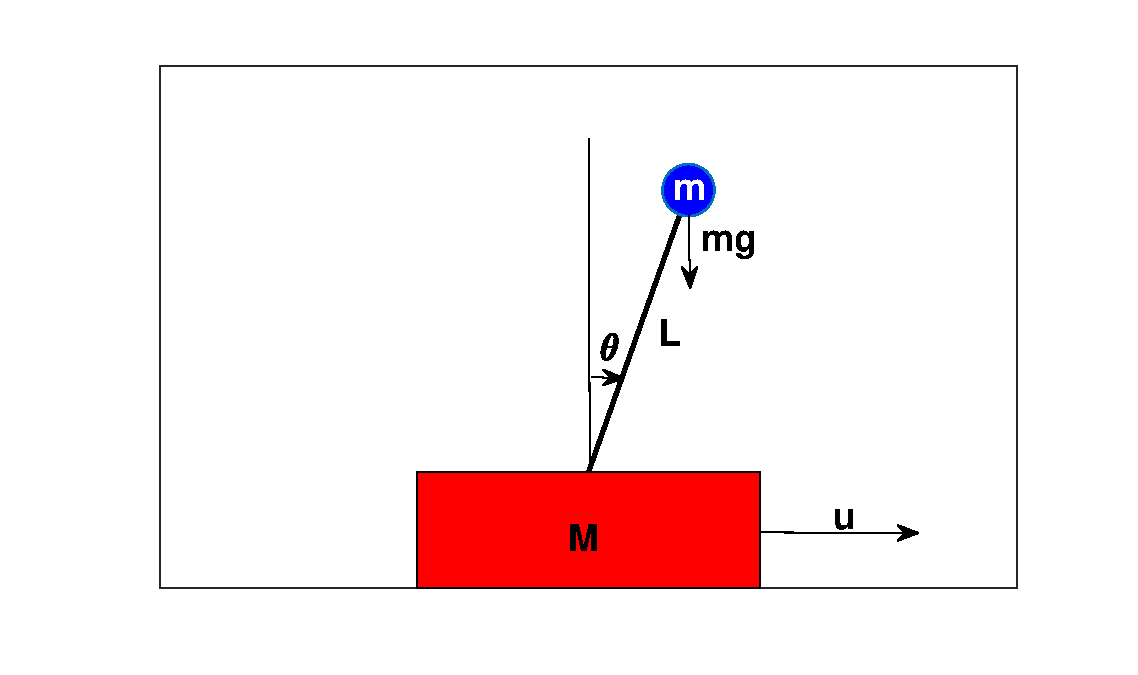
\includegraphics[width=\textwidth]{bloque.eps}

\hspace{12mm}  $ M =1\text{kg}\ m = 0.1\text{kg}\ L = 0.5\text{m}\  g = 10 \text{m/s}^2 $
\end{minipage}
\begin{enumerate}
\item \label{crtl} Construir el sistema linealizado en variables de estado, y comprobar analíticamente que se trata de una sistema inestable. Obtener la evolución de la salida del sistema para condiciones iniciales $\theta \neq 0$. Emplear para ello un ángulo pequeño para que la linealización realizada sea una aproximación válida.
\item Construye un sistema de control por realimentación de estados y comprueba que el sistema se estabiliza en la posición de equilibrio: $x_1 = 0, x_2 = 0$ para una condición inicial $x(0) =[0.4;1;0;0]$. Coloca los polos en $-1$; $ -2+0.5j$; $ -2-0.5j$; $-3$.

\item Supón que solo es posible conocer la posición del bloque. Diseña un sistema de control por realimentación de estados estimados, que permita estabilizar el sistema en su posicion de equilibrio. Comprueba que funciona correctamente en las mismas condiciones del apartado \ref{crtl}). Emplea para el observador como condiciones iniciales $\hat{x}(0) = [0,1,0,0]$.

\item Añadir al sistema de control diseñado acción integral, Emplear para este cálculo $y = x_2$ como única salida del sistema.
Vuelve a obtener la respuesta para un valor de la posición final del bloque $x=2$. Demuestra que no es posible aplicar control integral a la vez a las variables $x_1$ y $x_2$.
\end{enumerate}
\end{enumerate}

\section{Segundo Parcial}
\begin{enumerate}
\item El sistema,\footnote{\textbf{Si estás haciendo el final, contesta solo a esta pregunta.}},
\begin{equation}\label{eq1}
\begin{split}
\dot x_1 = -x_1^2 + \frac{1}{x_2}\\
\dot x_2 = \frac{x_1}{x_2} -1
\end{split},
\end{equation}
$x_1,x_2 \in \mathbb{R_+}$, representa un modelo de congestión de una red de comunicaciones. 	
	\begin{enumerate}
	\item (1 punto) Obtener los puntos de equilibrio del sistema, 			linealizar en torno a ellos y discutir su estabilidad.
	\item \label{apb} (2 puntos)  Emplea el criterio de estabilidad 		de Lyapunov del sistema linealizado, para obtener un función de 		Lyapunov y úsala para  estudiar la estabilidad del sistema no 		l	ineal. (Nota: puede ayudar realizar un dibujo de las componentes 		de la derivada de Lyapunov.)
	\item (2 puntos) Resuelve numéricamente la ecuación (\ref{eq1}), 		Para distintos valores de las condiciones iniciales, y obtén un 		diagrama de fases del sistema. Comprueba que los resultados son 		coherentes con el análisis realizado en los apartados anteriores.
	\end{enumerate}
	

\item Dado el sistema,
\begin{equation}\label{eq2}
\begin{split}
\dot x_1 &= x_2\\
\dot x_2 &= -x_1 - x_2(x_1^2+b)+u,
\end{split}
\end{equation} donde $[x_1,x_2]^T \in \mathbb{R}^2$, $b \in \mathbb{R} = cte$ y $u \in \mathbb{R}$ es una entrada al sistema,  y empleando la función de Lyapunov:
\begin{equation}
V = \frac{x_1^2 + x_2^2}{2}.
\end{equation}
\begin{enumerate}
\item (1 punto) Estudia la estabilidad de su único punto de equilibrio en función de valor de $b$.
\item \label{rea}(2 puntos) Comprueba que es posible recuperar la estabilidad del punto de equilibrio para $b\leq 0$  empleando una realimentación de estados de la forma $u = -Kx_2$.
 
\item (2 puntos) Tomando $b=-1$, resuelve numéricamente la ecuación (\ref{eq2}) y obtén un diagrama de fases, suponiendo una realimentación de estados como la descrita en el apartado \ref{rea}). Elige $K$ de modo el punto de equilibrio sea asintóticamente estable $\forall \  [x_1,x_2]^T \in \mathbb{R}^2$. 
\end{enumerate}
\end{enumerate}

\end{document}
